\section{Overview}



%\subsection{Pipeline Overview}

%\subsection{The Joint Loss Function}


% Our pipeline is as follows (Fig.~\ref{fig:arch_content}):
Our pipeline consists of the following steps (illustrated in Fig.~\ref{fig:arch_content}):

\begin{enumerate}
\item Fit a 3D model to extract static albedo textures from each frame in the source video sequence and the single RGB target image (Section 4).
\item Infer dynamic textures and retarget the per-frame texture expressions from the source video frames onto the target image texture using a generative adversarial framework (Section 5).
\item Composite the target mesh with the generated dynamic textures into each frame in the source video (Section 6).
\end{enumerate}

% \vfill\eject

\section{Fitting the Face Model}


We model the face shape $S$ and albedo as a multilinear PCA model with $n = 53k$ vertices and $106k$ faces:
\begin{equation}
S(\beta_{id}, \beta_{exp}) = \hat{S} + B_{id}\beta_{id} + B_{exp} \beta_{exp}
\end{equation}
\begin{equation}
I(\alpha_{alb}) = \hat{I} + A_{alb} * \alpha_{alb}
\end{equation}
The identity and expression are represented as a multivariate normal distribution with $B_{id} \in \mathbf{R}^{3n \times 80} $, $B_{exp} \in \mathbf{R}^{3n \times 29}$ and $A_{alb} \in \mathbf{R}^{3n \times 80}$.  The dimensions of the mean shape are $\hat{S} = \hat{S}_{id} + \hat{S}_{exp} \in \mathbf{R}^{3n}$, and the mean albedo is given by $\hat{I} \in \mathbf{R}^{3n}$.  The standard deviations are given by: $\sigma_{id} \in \mathbf{R}^{80}$, $\sigma_{exp} \in \mathbf{R}^{29}$ and $\sigma_{alb} \in \mathbf{R}^{80}$.

We use the Basel Face Model ~\cite{blanz1999} for $B_{id}$, $A_{alb}$, $\hat{S}$ and $\hat{I}$ as well as FaceWarehouse ~\cite{cao2014facewarehouse} for $B_{exp}$. We model the illumination using second order Spherical Harmonics and assume Lambertian surface reflectance.  We denote the illumination as $L \in \mathbf{R}^{27}$.  

Following the optimization scheme of ~\cite{f2f}, we jointly solve for all the unknowns $\textbf{Y} = \{ S, I, R, t, P, L \}$ leveraging the Gauss-Newton method applied to iteratively re-weighted least squares with three levels of image pyramid, where P are the camera parameters. One can refer to ~\cite{f2f} for details of this optimization.  In short, our objective function is:
\begin{equation}
E(\textbf{Y}) = w_{col} E_{col}(\textbf{Y}) + w_{lan} E_{lan}(\textbf{Y}) + w_{reg}E_{reg}(\textbf{Y})
\end{equation}
We use energy weights $w_{col} = 1$, $w_{lan} = 10$ and $w_{reg} = 2.5 \times 10^{-5}$.  
The photo-consistency term is given by 
\begin{equation}
E_{col}(\textbf{Y}) = \frac{1}{| M | } \sum_{p \in M}  ||C_{gt}(p) - C_{render}(p)||_2
\end{equation}
 where $C_{gt}$ is the input image and $C_{render}$ is the synthesized image.  $p \in M$ denotes pixel visibility in the source image.  
The landmark term is given by: 
\begin{equation}
E_{lan}(\textbf{Y}) = \frac{1}{|F|} \sum_{f_i \in F}  || f_i - \Pi_P(RS_i + t) ||_2^2
\end{equation}
 where $f_i \in F$ is a 2D facial feature following the method presented in ~\cite{kazemi2014one}.  
The regularization $E_{reg}$ term ensures that faces stay close to the normal distribution.  This term prevents degenerative faces when performing the fitting:
\begin{equation}
E_{reg}(\textbf{Y}) = \sum_{i = 1}^{80} [ (\frac{\beta_{id, i}}{\sigma_{id,i}})^2 + (\frac{\alpha_{alb, i}}{\sigma_{alb, i}})^2] + \sum_{i =1}^{29} ( \frac{\beta_{exp,i}}{\sigma_{exp,i}})^2
\end{equation}

\section{ Dynamic Texture Synthesis}

\subsection{Deep Learning Framework}

\begin{figure*}[th]
	\centering
	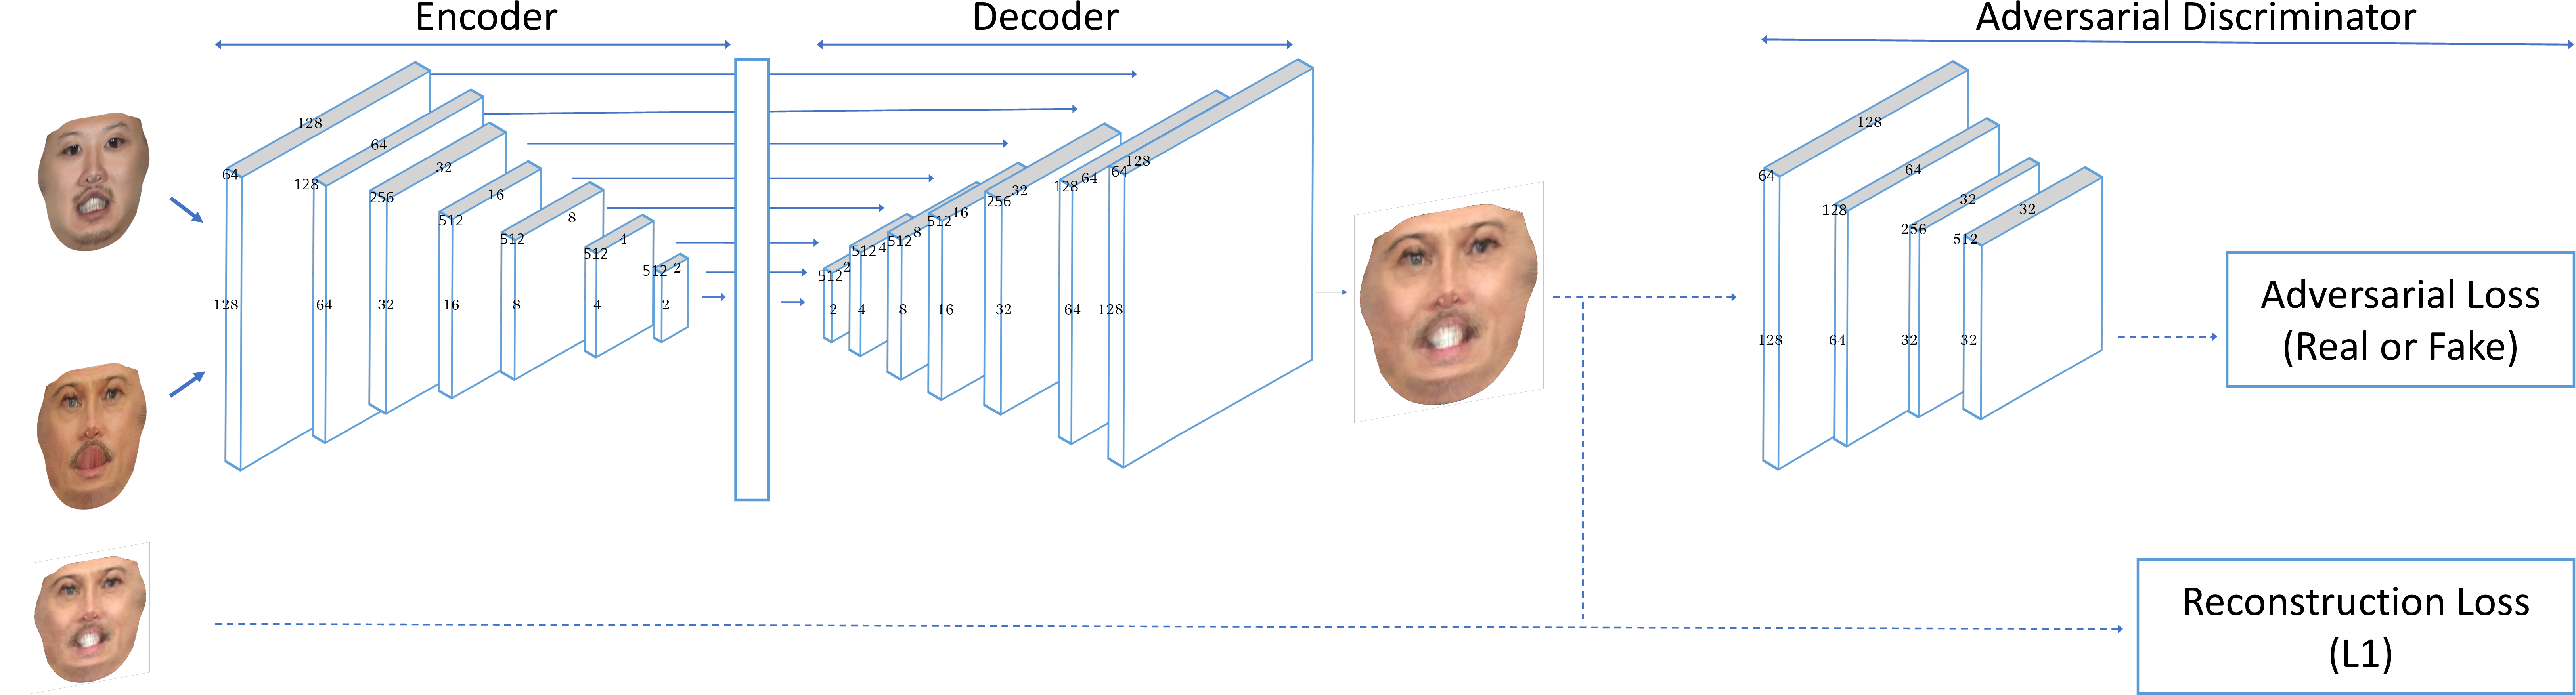
\includegraphics[width=1\linewidth]{figures/network/network.png}
	\caption{The network architecture. The encoder takes as input the identity texture and the expression texture, and the decoder outputs the dynamic texture. The adversarial discriminator is used during training to judge whether the output texture looks real or not.}\label{fig:network}
	\vspace{-0.15in}
\end{figure*}

The core of our dynamic texture synthesis pipeline for inferring fine details is a Conditional Generative Adversarial Network used to infer deformations from a source texture onto a target texture.
Broadly speaking, a Generative Adversarial Network (GAN) $G$ is a function which produces ``realistic'' output from a noise vector.  
That is, given a distribution $M$, a variable $z \sim M$, and a set of ground truth ``real'' examples $X$,  we would like $G(z)$ to be indistinguishable between 
any $x \sim X$.  Formally, by indistinguishable we mean to say that the generator function fools as best as possible a discriminator function, $D$, 
trained precisely to separate the generated output $G(z)$ from the real output drawn from $X$. A conditional GAN, on the other hand, takes as input both the noise vector $z$, along with additional input $y$ in order to produce the output $x$.    
Notice that $y$ and $x$ are not necessarily from the same set.  

In our setting, we attempt to learn a target texture deformation given a source texture deformation.  
That is, given a source texture $U_{source}$ that encodes a given expression, we would like to transfer this expression to a neutral-pose target texture $N_{target}$.  
For example, the source texture expression might contain a wrinkle on the left cheek that we would like to synthesize onto the target neutral texture. 
In this case, the output is $U_{target}$, the target texture with the wrinkle, and we are conditioning on $U_{source}$ and $N_{target}$.  


Note that neural networks are inclined to be heavily affected by noise and variation within the training corpus.  For this reason, we work in the UV texture space of the captured facial albedos.  This provides many benefits during training.  First of all, it minimizes variations in the input due to factors such as lighting, image background and head pose. In UV space, the mouth, eyes, and nose are in the exact same location in each image - the only thing that changes is the content of those locations. Working in this space makes it possible to retarget mouth motion, blinking, scrunching, and various other skin deformations that would be much harder to learn otherwise.  


\subsection{Loss Function}

The energy function we minimize is given by 
\begin{equation} \label{eqn:1}
\begin{split}
L_{GAN}(G,D)& = E_{{x,y}\sim p_{data}({x,y}),z\sim p_z{z}}[\log D({t})]\\
& +E_{{x,y}\sim p_{data}(x),z\sim p_z(z)}[\log(1-D(G(x,z)))] 
\end{split}
\end{equation}

In our formulation, $x$ is the pair $(U_{source}, N_{target})$ and $y$ is given by $U_{target}$.  
In addition to this energy, the generator $G$ also attempts to minimize the reconstruction loss to the target $y$ in the $\ell_1$ sense.  
That is, $L_{recon}(G)= E[\parallel y-G({x,y},z)\parallel_1]$ ~\cite{pix2pix}.

$G$ attempts to minimize this objective while $D$ attempts to maximize it.  In other words:
$ G_{opt}=\text{arg}\min\max L_{cGAN}(G,D)+\lambda L_{\ell_1}(G)$, where $\mu$ 
encodes the relative weighting of the different errors ~\cite{pix2pix}.  In our implementation of the conditional GAN, 
we do not input any noise during generation, but otherwise the optimization program is accurate.  We set $\mu = 0.001$ in all experiments. 
This parameter can be viewed as a balancing between the need to reconstruct accurate wrinkles with the need to have the final texture
remain "realistic".  

\subsection{Network Architecture}


We use a similar architecture as \cite{pix2pix}. 
First, we concatenate the driver expression and the neutral target identity, $(U_{source}, N_{target})$, along their color-channel dimension as input.
The generator output is the target expression $y$, which is the expression transferred from the source to target texture.

Second, we use a masked prior to define the $\ell_1$ and adversarial loss. 
The mask is applied on the $\ell_1$ loss such that the the loss around the mouth and eye regions is ten times higher than in other areas - we
do this because wrinkles, blinking, and most texture deformations are a lot more prevalent in these areas.  
For the discriminator, we adopt a Markovian Discriminator 
(PatchGAN) with patch size set to $70 \times 70$. We found that adding skip connections between
encoder layers and decoder layers, skipping around the code layer, greatly reduces noise in the output image. 
%Finally, we do not input any 
The parameters are
optimized using ADAM with back-propagation. Our input and output resolution are $256\times 256$.


%%\begin{eqnarray*}
%%G^*&=&arg\min\max L_{cGAN}(G,D)+\lambda L_{L1}(G) \\
%%L_{L1}(G)&=& E[M\cdot\parallel y-G({x,y},z)\parallel_1] \\
%%L_{GAN}(G,D)&=& E_{{x,y}\sim p_{data}({x,y}),z\sim p_z{z}}[\log D({t})]+E_{{x,y}\sim p_{data}(x),z\sim p_z(z)}[\log(1-D(G(x,z)))]
%%\label{eqn:1}
%%\end{eqnarray*}

\subsection{Mouth Synthesis}

\begin{figure}[h]
	\centering
	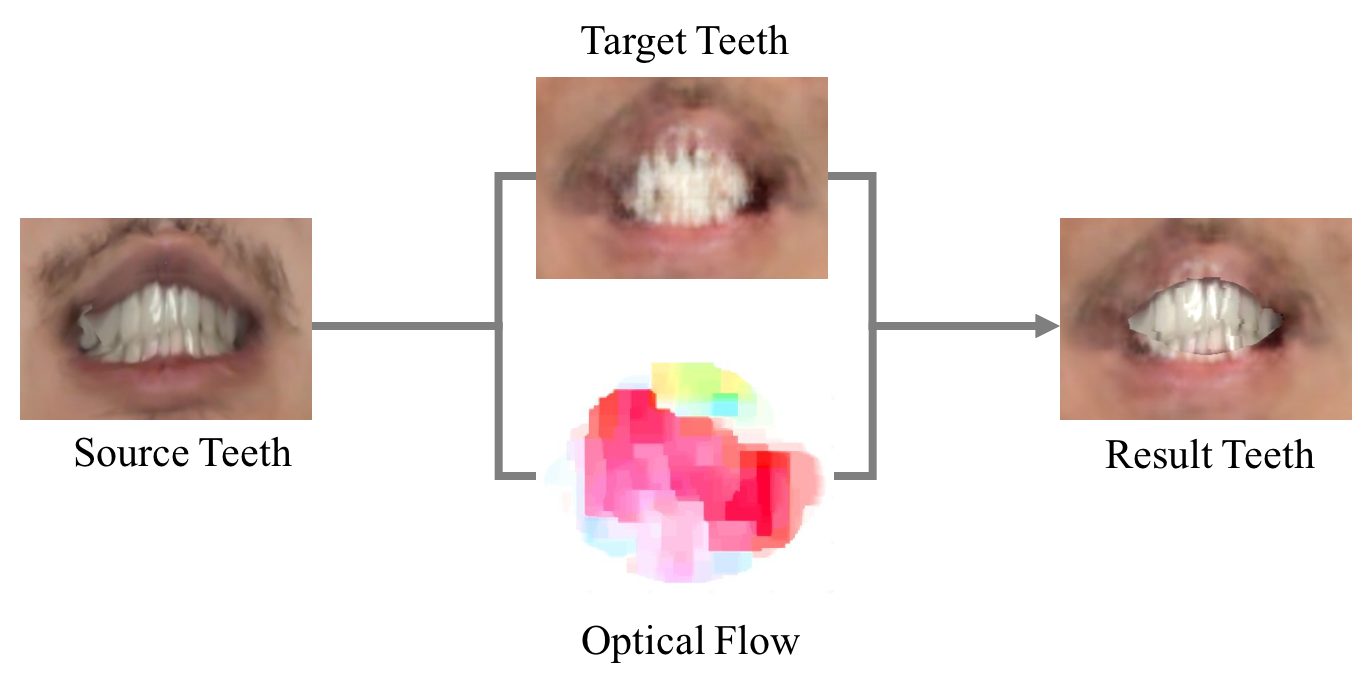
\includegraphics[width=1\linewidth]{figures/flow/opticalflow2.png}
	\caption{Visualization of flow-upsampling from source mouth to low-resolution inferred mouth.  Left is source mouth, top is target mouth, bottom is flow field, right is final result.}\label{fig:flow}
	\vspace{-0.05in}
\end{figure}
We model the mouth interior region as a part of the UV texture.  When the mouth is closed, the area between the lips get projected onto this area to
make a pink color.  When the mouth is open, the mouth interior, including the teeth and tongue, are projected to this region (Fig.~\ref{fig:flow}).  

Using our deep-learning framework, we are able to transfer open-mouth expressions onto the closed-mouth neutral target textures and infer the
inner mouth region.  However, due to lack of training data for the mouth interior, the inferred texture here tends to be of rather low resolution.  In order
to improve this area, we use SIFT-Flow ~\cite{siftflow} to redraw the target mouth using the source mouth for each frame.  In particular, after
computing SIFT features at the pixel level, we perform matching based on the following energy term:
\begin{equation}
\begin{split}
E(w)& = \sum_p \min (||s_1(p) − s_2(p + w(p))||_1, t)  \\
&\hspace{-6mm} +\sum \eta(|u(p)| + |v(p)|)  \\
&\hspace{-6mm} +\sum_{(p,q) \in \epsilon} min(\alpha |u(p) - u(q)|, d) + min(\alpha|v(p) - v(q)|, d)
\end{split}
\end{equation}
The terms in the equation are, in order, the data term, the small displacement term, and the spatial regularization term ~\cite{sift}, 
where $w(p) = (u(p), v(p))$ is the flow vector at a point $p = (x,y)$, and $s_1$ and $s_2$ are the sift features
computed for either image 1 or image 2 at the point $p$.  The second and third term regularize the matching by pushing
nearby points to get mapped to each other.

Inferring the inner mouth also has the added benefit of improving the lip texture around the mouth during tracking failure of the original video: tracking of tight-lipped
expressions such as kissing often fail and the lip texture gets projected to the interior region in UV space.  During rendering, this causes
the lips to be thinner than they should be, which gives an unnatural appearance.  By inferring this inner-mouth region, we are able to synthesize realistic 
kissing faces on the target even when lip tracking fails on the source.

%\subsection{Fitting to Video Sequence}

%We adopt a similar optimization scheme as ~\cite{f2f} to obtain the per-frame mesh and per-frame texture of the source video sequence at run-time.  In particular:

%%IMPLEMENTATION DETAILS OF F2F

%Using the per-frame texture, we synthesize per-frame textures and mouth flows using the above framework on the single RGB target image, and then
%are able render a realistic animation of the target.  

\section{Video Face Replacement via Blending}

Once we have the per-frame textures and retargeted mesh, we are also able to transfer the target appearance back onto the source video
sequence for a detailed and realistic animation (Fig.~\ref{fig:blend}). We use a graph-cut approach similar to ~\cite{replace} in order 
to achieve this.  In particular, for blending the retargeted faces to the source video in a photorealistic manner,
we first find a graph-cut to partition each frame into two regions, which determines whether 
a pixel comes from the frame in the source video or the image of the rendered retargeted face model(Fig.~\ref{fig:blend}a-c). 
We then linearly blend the target and source regions of the images along the seam to achieve a smooth and realistic result (Fig.~\ref{fig:blend}d).
 
\begin{figure}[t]
  \centering
  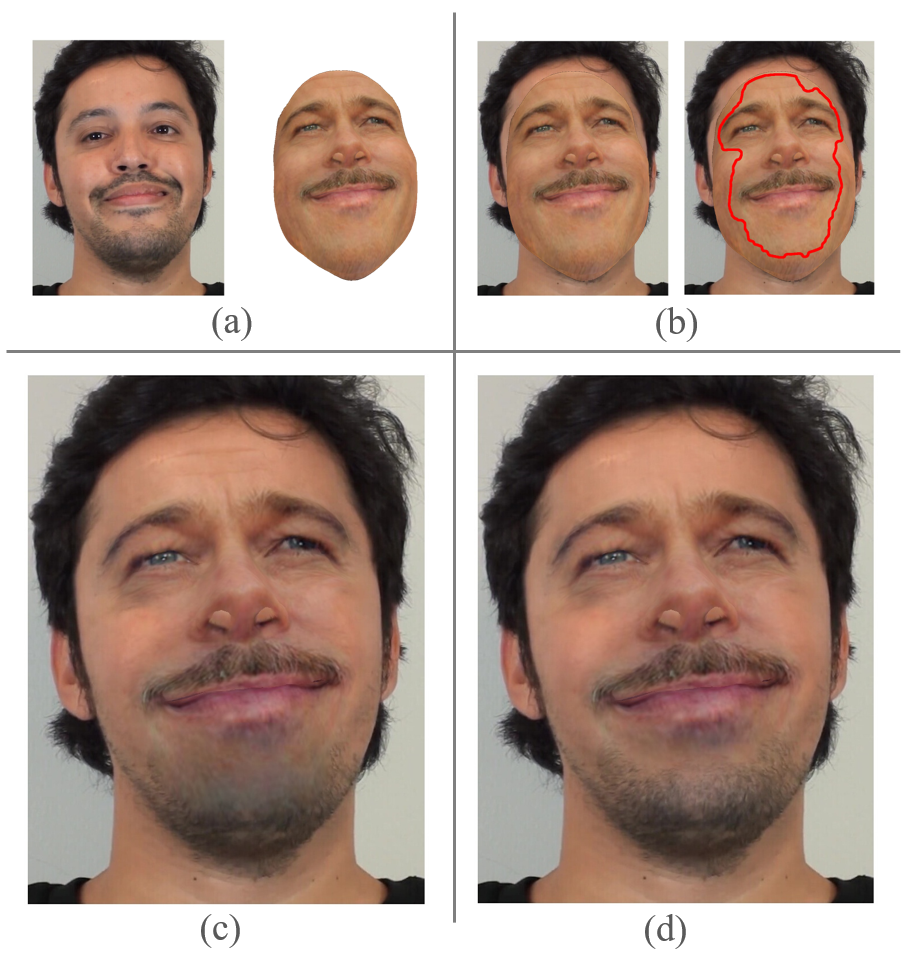
\includegraphics[width=0.6\linewidth]{figures/blending/blending.pdf}
  \caption{a) The input consists of the frames of the source video (left) and the rendered retargeted mesh (right). b) Naively projecting all of the target mesh's vertices onto the source frame results in an unrealistic and incoherent result (left) when a more optimal partition is outlined in red on the image on the right. 
	c) The composition of the two images using the optimal scene.
	d) Linearly blending the pixels along the seam gives a smooth and realistic result.}
	\label{fig:blend}
  \vspace{-0.15in}
\end{figure}



\subsection{Graph-Cut}
Similar to ~\cite{replace}, 
we optimize the partition so as to ensure spatial coherence coherence between neighboring pixel values
and temporal coherence between frames. 


If we naively project the mesh back onto the frame of the source video, as seen in the left-hand image of Fig~\ref{fig:blend}b, the result is not smooth or realistic. 
In order to maintain spatial coherence across large variations in pose and expression, 
 we construct a graph-cut problem on each of the frames in the source video and their corresponding retargeted mesh as in ~\cite{graphcut}. For each frame, the graph cut algorithm labels each vertex on the mesh as either a source vertex or target vertex in a manner that minimizes the difference in pixel values across neighboring vertices, as shown on the right-hand image of Fig.~\ref{fig:blend}b. We then project the seam of the labeled mesh onto the image (Fig.~\ref{fig:blend}c). 

The nodes of the graph represent the vertices on the mesh for each frame in the source video. 
Let each vertex be denoted as $V_{t,i}$, where $t$ refers to the $t$th frame, and $i$ refers to the $i$th vertex on the mesh. 
%and construct the following graph to calculate the seam in the rest region.

In order to minimize the difference between source and target pixels along the seam, for each frame, we set weights on the graph for each edge between each pair of vertices $V_{t,u}$ and  $V_{t,v}$ that share an edge on the mesh as:
\begin{equation}
\begin{split}
W_m(V_{t,u}, V_{t,v}) = & \|I_{s}(V_{t,u})-I_{s}(V_{t,v})\|\\
& + \|I_{t}(V_{t,u})-I_{t}(V_{t, v})\| 
\end{split}
\end{equation}

 $I_{s}$is the source image, $I_{w}$ is the target image, $I_{s}(V)$ is the color at the pixel where $V$ is projected onto the source frame, and $I_{t}(V)$ is the color at the pixel V is projected onto in the rendered target image.
 For temporal coherence, we set edges between vertices $V_{t,i}$ and $V_{t+1,i}$ for all $i$ and $t$, with weight as:
\begin{equation}
\begin{split}
W_f(V_{t,i}, V_{t+1,i})& = \lambda \|I_{s}(V_{t,i})-I_{s}(V_{t+1,i} +1)\|^{-1}\\
              & + \|I_{t}(V_{t,i})-I_{t}(V_{t+1,i} + 1)\|^{-1}
\end{split}
\end{equation}

After computing the seam, we can composite the target appearance onto the source video and linearly blend the pixels across the seam for a realistic novel reenactment.  





